\documentclass{beamer}
\mode<presentation>
\usetheme{Boadilla}

\usepackage{amsmath,amssymb}
\usepackage{graphicx}
\usepackage{siunitx}
\sisetup{per-mode=symbol}
\usepackage{gvv}
\usepackage{listings}
\usepackage{xcolor}

% Code style
\lstset{
  basicstyle=\ttfamily\scriptsize,
  breaklines=true,
  frame=single,
  numbers=left,
  numberstyle=\tiny,
  keywordstyle=\color{blue},
  commentstyle=\color{green!50!black},
  stringstyle=\color{red!60!black},
  showstringspaces=false
}

\title{Matrix 1.7.1}
\author{ai25btech11015 -- M Sai Rithik}
\date{}

\begin{document}
\frame{\titlepage}

\begin{frame}{Question}
Find the unit vector along $\Vec{PQ}$, where $P=(2,1,-1)$ and $Q=(4,4,-7)$.  
Name the unit vector $\Vec{OA}$, where $O$ is the origin.
\end{frame}

\begin{frame}{Step 1: Vector $\Vec{PQ}$}
\[
P = \myvec{2 \\ 1 \\ -1}, 
\quad Q = \myvec{4 \\ 4 \\ -7}.
\]
\begin{equation}
\Vec{PQ} = Q - P = \myvec{2 \\ 3 \\ -6}
\end{equation}
\end{frame}

\begin{frame}{Step 2: Magnitude of $\Vec{PQ}$}
\begin{equation}
\|\Vec{PQ}\| = \sqrt{2^2 + 3^2 + (-6)^2}
= \sqrt{49} = 7
\end{equation}
\end{frame}

\begin{frame}{Step 3: Unit vector}
\begin{equation}
\Vec{OA} = \frac{\Vec{PQ}}{\|\Vec{PQ}\|}
= \frac{1}{7}\myvec{2 \\ 3 \\ -6}
\end{equation}
\end{frame}

\begin{frame}{Final Answer}
\[
\boxed{\Vec{OA} = \tfrac{1}{7}\myvec{2 \\ 3 \\ -6}}
\]

\begin{figure}[h!]
    \centering
    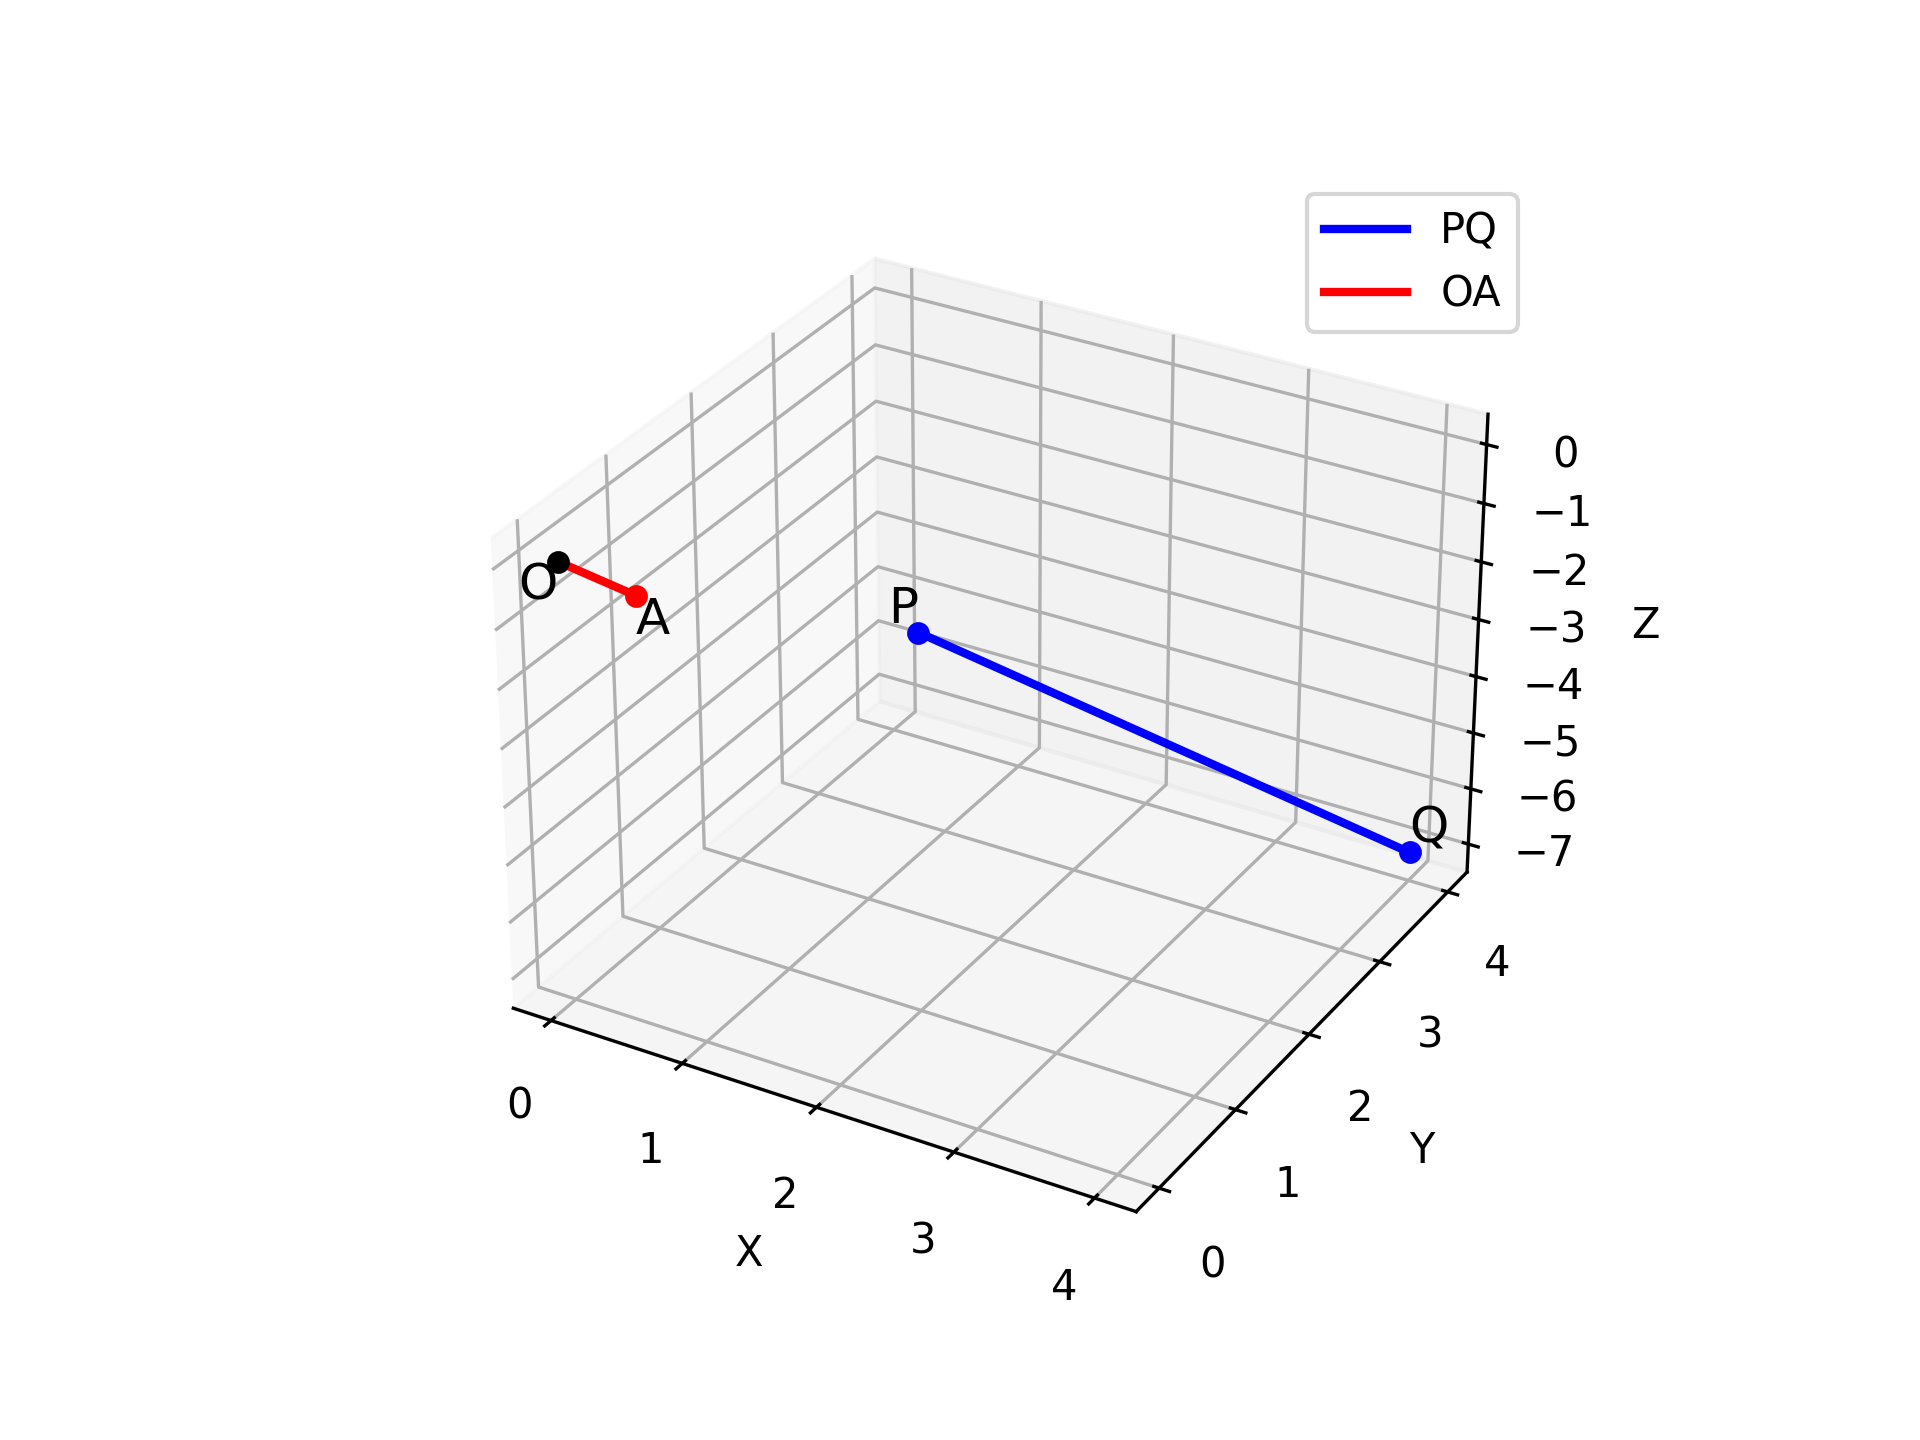
\includegraphics[width=0.6\linewidth]{figs/fig.png}
    \caption{Unit vector $\Vec{OA}$ along $\Vec{PQ}$}
\end{figure}
\end{frame}

% -------- C Code Split Across Frames ----------
\begin{frame}[fragile]
    \frametitle{C Code}
    \begin{lstlisting}[language=C]
#include <stdio.h>
#include <math.h>

int main() {
    // Coordinates of P and Q
    double P[3] = {2, 1, -1};
    double Q[3] = {4, 4, -7};

    // Vector PQ = Q - P
    double PQ[3];
    for (int i = 0; i < 3; i++) {
        PQ[i] = Q[i] - P[i];
    }

    // Magnitude of PQ
    double magnitude = sqrt(PQ[0]*PQ[0] + 
                            PQ[1]*PQ[1] + 
                            PQ[2]*PQ[2]);

    // Unit vector along PQ
    double unit[3];
    for (int i = 0; i < 3; i++) {
        unit[i] = PQ[i] / magnitude;
    }
    \end{lstlisting}
\end{frame}

\begin{frame}[fragile]
    \frametitle{C Code}
    \begin{lstlisting}[language=C]
    // Print the unit vector
    printf("Unit vector along PQ: (%.4f, %.4f, %.4f)\n",
           unit[0], unit[1], unit[2]);

    // Write P, Q, and the unit vector to the file
    FILE *fp = fopen("unit_vector.dat", "w");
    if (fp != NULL) {
        fprintf(fp, "%.6f %.6f %.6f\n", P[0], P[1], P[2]);
        fprintf(fp, "%.6f %.6f %.6f\n", Q[0], Q[1], Q[2]);
        fprintf(fp, "%.6f %.6f %.6f\n", unit[0], unit[1], unit[2]);
        fclose(fp);
        printf("Coordinates written to unit_vector.dat\n");
    } else {
        printf("Error opening file for writing.\n");
    }

    return 0;
}
    \end{lstlisting}
\end{frame}

% -------- Python Code Split Across Frames ----------
\begin{frame}[fragile]
    \frametitle{Python Code}
    \begin{lstlisting}[language=Python]
import numpy as np
import matplotlib.pyplot as plt

# Read coordinates from unit_vector.dat
coords = []
with open('unit_vector.dat', 'r') as f:
    for line in f:
        if line.strip():
            coords.append([float(x) for x in line.strip().split()])

P = np.array(coords[0][:2])
Q = np.array(coords[1][:2])
A = np.array(coords[2][:2])
O = np.array([0, 0, 0])

# Create 3D plot
fig = plt.figure()
ax = fig.add_subplot(111, projection='3d')

# Plot PQ in 3D
ax.plot([coords[0][0], coords[1][0]],
        [coords[0][1], coords[1][1]],
        [coords[0][2], coords[1][2]],
        color='blue', label='PQ', linewidth=2)
    \end{lstlisting}
\end{frame}

\begin{frame}[fragile]
    \frametitle{Python Code}
    \begin{lstlisting}[language=Python]
# Plot OA in 3D
ax.plot([0, coords[2][0]],
        [0, coords[2][1]],
        [0, coords[2][2]],
        color='red', label='OA', linewidth=2)

# Label points
ax.scatter(coords[0][0], coords[0][1], coords[0][2], color='blue')
ax.text(coords[0][0], coords[0][1], coords[0][2], 'P')
ax.scatter(coords[1][0], coords[1][1], coords[1][2], color='blue')
ax.text(coords[1][0], coords[1][1], coords[1][2], 'Q')
ax.scatter(coords[2][0], coords[2][1], coords[2][2], color='red')
ax.text(coords[2][0], coords[2][1], coords[2][2], 'A')

ax.scatter(0, 0, 0, color='black')
ax.text(0, 0, 0, 'O')

ax.set_xlabel('X')
ax.set_ylabel('Y')
ax.set_zlabel('Z')
ax.legend()
ax.grid(True, linestyle='--', alpha=0.5)

# Save figure
fig.savefig('../figs/fig.png', dpi=300)
    \end{lstlisting}
\end{frame}

\end{document}
